\documentclass[11pt]{article}
\usepackage{fullpage}
\usepackage{algorithm}
\usepackage[noend]{algorithmic}
\usepackage{enumerate}
\usepackage{amsmath,amssymb,amsthm}
\usepackage{stackrel}
\usepackage[english]{babel}
\usepackage[utf8x]{inputenc}
\usepackage{amsmath}
\usepackage{tikz}
\usetikzlibrary{arrows,automata}

% Helpful Shortcuts
\newcommand{\bc}[1]{{\quad \text{(#1)}}} 	% Justification in math env
\newcommand{\st}{{\text{ such that }}} 							   % Math env
\newcommand{\abs}[1]{{ |#1 |}} 							% Absolute value / Cardinality
\newcommand{\bld}[2]{\noindent\textbf{#1:}\hspace{0.1in}#2$  $\bigskip} % Headings
\newcommand{\notimplies}{%
	\mathrel{{\ooalign{\hidewidth$\not\phantom{=}$\hidewidth\cr$\implies$}}}}
\newcommand{\linesep}{\noindent\bigskip\rule{17cm}{0.1mm}\bigskip} % Horizontal Line

% These define new environments / formats for lemmas, definitions, running time, etc.
\newtheorem{lemma}{Lemma}
\newtheorem{definition}{Definition}
\newtheorem{notation}{Notation}
\newtheorem*{claim}{Claim}
\newtheorem{observation}{Observation}
\newtheorem{conjecture}[lemma]{Conjecture}
\newtheorem{theorem}[lemma]{Theorem}
\newtheorem{corollary}[lemma]{Corollary}
\newtheorem{proposition}[lemma]{Proposition}
\newtheorem*{rt}{Running Time}

% These define nice ways to format P and OPT (use \P or \opt)
\def\P{\ensuremath{$ \mathcal{P} $}}
\def\opt{\ensuremath{\textsc{opt}}}
\renewcommand{\labelenumi}{\bf \alph{enumi}.}

\renewcommand\maketitle{
	\begin{center}
		\begin{tabular*}{6.44in}{l @{\extracolsep{\fill}}c r}
			\bfseries  &  & \bfseries CSCI 383 Spring 2019 \\
			\bfseries&  & \bfseries  Homework \#4 Solutions  \\
			\bfseries   &   &  \bfseries Kai Ting Keshia Yap\\ 
		\end{tabular*}
\end{center} }

\begin{document}
	\maketitle
	
	\noindent Honor Code: I affirm that I adhered to the Honor Code in this assignment. Keshia Yap
	
	\subsection*{Part  2: Closed Encounters}
	Let $ N:=\{a^nb^n\mid n\geq 0\} $, which we showed in class to be a nonregular language. We will show that the following languages are nonregular by closure properties of regular languages.
	
	\begin{enumerate}
		\item $ L_4=\{a^{p-1}\mid p\text{ is prime}\} $
		\begin{proof}
			Observe that $A= \{a\} $ is a regular language given by the DFA:\\
			\begin{center}
			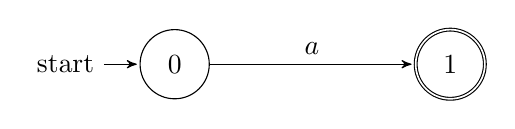
\begin{tikzpicture}[->,>=stealth',shorten >=1pt,auto,node distance=3.5cm,scale = 1,transform shape]
			\node[state,initial] (0) {$0$};
			\node[state,accepting] (1) [right of=0] {$1$};
			\path (0) edge              node {$a$} (1);
			\end{tikzpicture}
			\end{center}
			
			Since regular languages are closed under concatenation, if $ L_4 $ were regular then $ aL_4=\{a^p\mid p\text{ is prime}\}=L_3$ would be regular, contradicting Part 1c. of this homework.
		\end{proof}
		\item $ L_5=\{a^{2n+1}b^{2n+1}\mid n\geq 0\} $
		\begin{proof}
			Note that $ L_5\cup aL_5b\cup \{\epsilon\} =N$. We know that regular languages are closed under concatenation and union, and that $A= \{a\} $, $B= \{b\} $, $\{\varepsilon\} $ are a regular languages given by DFAs similar to the one in Part 2a. If $ L_5 $ were regular then $ N $ would be regular. Contradiction.
		\end{proof}
		\item $ L_6=\{x\in \{(,)\}^*\mid x\text{ is balanced}\} $
		\begin{proof}
			Replace $(\mapsto a $ and $ )\mapsto b $ to get $L_6'= \{x\in\{a,b\}\mid \#a(x_n)\geq \#b(x_n) \forall n, \#a(x)=\#b(x)\} $ where $ x_n $ refers to the first $ n $ characters of $ x $ and $ \#c(x) $ denotes the number of characters $ c $ in string $ x $. Let $ C:=\{a^mb^n\mid m,n\geq 0\} $. This is regular as we showed it in class. Suppose that $ L_6 $ is regular. Then $ L_6'\cap C=N$ is regular. Contradiction.
		\end{proof}
		\item $ L_7=\{a^nb^mc^k\mid n,m,k\geq 0\text{ and }n+m=k\} $
		\begin{proof}
			Consider the language of $ L_7 $ where all the $ b $'s are replaced with $ a $'s and all the $ c $'s are replaced with $ b $'s. This language is 
			\begin{align*}
				 D:&= \{a^n a^mb^k\mid n,m,k\geq 0\text{ and }n+m=k\} \\
				 &=\{a^{n+m}b^k\mid n,m,k\geq 0\text{ and }n+m=k\} \\
				 &=\{a^kb^k\mid k\geq 0\}
			\end{align*}
			Since languages are closed under character replacement, if $ L_7 $ were regular then $ D =N$ would be regular, again contradicting what we showed in class.
		\end{proof}
	\end{enumerate}
	

\end{document}